%======================================================================
% GMI-08 Metricka struktura.pdf
%======================================================================
\section{Metrika}
\strana{GMI-08-1}
\begin{itemize}[nosep]
  \item Metrický tenzor
  \item Riemanovské geometrie
  \item Lorentzovské geometrie
  \item Délka křivky
  \item Levi-Civitův tenzor a Hodgeův duál
  \item Killingovy vektory
\end{itemize}

%----------------------------------------------------------------------
\strana{GMI-08-2}
\subsection{Metrický tenzor} \pozn{Metr 1}

Geometrie
\begin{itemize}[nosep]
  \item[--] lze identifikovat se schopností měřit délky
  \item[--] vnitřní a vnější geom.
\end{itemize}

\begin{definice}[Metrický tenzor]
\kw{metrický tenzor} \quad $g_{\underline{ab}}\in\mathbb{T}^0_2M$
\begin{itemize}[nosep]
  \item[--] symetrický \hfill $g_{\underline{ab}} = g_{\underline{ba}}$
  \item[--] nedegenerovaný \hfill $\forall a\neq 0 \quad g_{\underline{a}\underline{n}}a^{\underline{n}}\neq 0$
\end{itemize}
\kw{inverzní metrika} \quad $g^{-1\,\underline{ab}}\in\mathcal{T}^2_0M$
\[
  \vzorec{g^{-1\,\underline{an}}g_{\underline{nb}} = g_{\underline{bn}}g^{-1\,\underline{na}} = \delta^{\underline{a}}_{\underline{b}}}
\]
\end{definice}

\begin{vysvetleni}[Metrika]
Metrika je v každém bodě symetrická bilineární forma na tečném prostoru; měří \uv{kvadrát délky} infinitezimálního posunutí, $\mathrm{d}s^2=g_{ab}\,\mathrm{d}x^a\mathrm{d}x^b$. Pozitivitu nepožadujeme, aby šlo zahrnout i prostoročas. Nedegenerovanost znamená, že zobrazení $a^n\mapsto g_{\underline{a}\underline{n}}a^{\underline{n}}$ je prosté, ve složkách $\det g_{ab}\neq0$, a proto existuje inverzní metrika $g^{-1}$ (ve složkách inverzní matice).
Podtržené indexy jsou abstraktní, nepodtržené jsou složky v bázi. Viz Krtouš, odd.~6.1, def.~D6.1.
\end{vysvetleni}

\kw{ortonormální báze}
\[
  e^{\underline{a}}_k\,e^{\underline{b}}_l\,g_{\underline{ab}} = \begin{cases} \pm1 & k = l \\ 0 & k\neq l\end{cases}
\]
\quad duální báze $e^k_{\underline{a}}$

\kw{signatura}
\begin{itemize}[nosep]
  \item[] počet vekt.\ v ortonorm.\ bázi se záp.\ \hfill kvadr.\ vel. \\
          \quad $e^{\underline{a}}_k e^{\underline{b}}_k g_{\underline{ab}} = -1$ \qquad\qquad $e^{\underline{a}}_l e^{\underline{b}}_l = +1$
  \item[] nezávisí na volbě báze
  \item[$\to$] signatura \quad $(\underbrace{-\,-\,\dots}_{m}\ \underbrace{+\,+\,\dots}_{p})$
  \item[] $\vzorec{\operatorname{sign} g = (-1)^m}$ $=$ součin znam.\ v signatuře
\end{itemize}

\kw{metrická báze}
\[
  g_{ab} = e^{\underline{m}}_a e^{\underline{n}}_b\,g_{\underline{mn}} = \text{konst.}
\]
\quad ortonorm.\ báze je metrická

\begin{vysvetleni}[Ortonormální báze a signatura]
Ortonormální báze (\uv{n-áda}, \uv{reper}) existuje vždy (Gramova--Schmidtova ortogonalizace). Počty vektorů s kvadrátem velikosti $-1$ a $+1$ na volbě báze nezávisí (Sylvestrův zákon setrvačnosti), a to je signatura $(m,p)$ s $m+p=d$. Vektory se záporným kvadrátem se píší první. Veličina $\operatorname{sign}g=(-1)^m$ je zároveň znaménkem $\det g_{ab}$ v libovolné bázi.
\uv{Metrická báze} je báze, v níž má metrika konstantní složky. Ortonormální báze je jejím speciálním případem se složkami $\operatorname{diag}(-1,\dots,-1,+1,\dots,+1)$.
Viz Krtouš, def.~D6.2, D6.3.
\end{vysvetleni}

%----------------------------------------------------------------------
\strana{GMI-08-3}
\subsubsection*{Zvyšování a snižování indexů} \pozn{Metr 2}
metrika $g$ definuje isomorf.\ $\mathbb{T}M$ a $\mathbb{T}^*M$
\begin{align*}
  a^{\underline{m}} &\to ({}^\flat a)_{\underline{m}} = g_{\underline{mn}}a^{\underline{n}} & a_n &= g_{nm}a^m \\
  \alpha_{\underline{m}} &\to ({}^\sharp\alpha)^{\underline{m}} = g^{-1\,\underline{mn}}\alpha_{\underline{n}} & \alpha^n &= g^{-1\,nm}\alpha_m
\end{align*}
budeme běžně vynechávat $\sharp$ a $\flat$, tj.\ \quad zřejmě
\[
  {}^\sharp g^{\underline{ab}} = g^{-1\,\underline{ab}} \qquad\text{tj.}\qquad {}^\sharp g^{ab} = g^{-1\,ab} = g^{ab}, \qquad g^{\underline{a}}{}_{\underline{b}} = \delta^{\underline{a}}_{\underline{b}}
\]

ortonormální báze
\[
  {}^\flat e_a = \pm e^a \qquad\qquad {}^\sharp e^a = \pm e_a
\]
\quad kde $\pm = \operatorname{sign}\big(e^{\underline{m}}_a \oprava{e^{\underline{n}}_a}{e^{\underline{n}}_b}\,g_{\underline{mn}}\big)$

riemanovská signatura $(+\,+\,\dots\,+)$ \\
\quad pro ort.\ bázi platí
\[
  {}^\sharp e^a = e_a \qquad\qquad a^m = a_m \qquad \Leftarrow\ g_{ab} = g^{ab} = \begin{bmatrix}1 & & \\ & 1 & \\ & & \ddots\end{bmatrix}
\]

\begin{vysvetleni}[Zvyšování a snižování indexů]
Nedegenerovaná metrika dává kanonický izomorfismus $\mathbb{T}M\cong\mathbb{T}^*M$: vektoru $a$ přiřadí 1-formu ${}^\flat a=g(a,\cdot)$ (\uv{snížení indexu}, $\flat$) a inverzní metrika provede opačný krok ($\sharp$). Běžná konvence pak značky vynechává a typ objektu se pozná jen podle polohy indexů ($a_n=g_{nm}a^m$). Proto je třeba hlídat \emph{pořadí} indexů i po zvednutí, např.\ $R^a{}_{bcd}$ vs.\ $R_{abcd}$. Inverzní metrika je pak $g^{ab}$ a se smíšenými indexy $g^a{}_b=\delta^a_b$.
V ortonormální bázi se složky s horním a dolním indexem liší nanejvýš znaménkem $\pm=\operatorname{sign}(g(e_a,e_a))$, v riemannovském případě se shodují. (V přepisu prvních dvou řádků jsou indexy srovnány podle originálu.)
Viz Krtouš, odd.~6.3, def.~D6.9, vztahy (6.5)--(6.9).
\end{vysvetleni}

%----------------------------------------------------------------------
\strana{GMI-08-4}
\subsection{Riemanovské geometrie} \pozn{Metr 3}

\begin{minipage}{0.6\textwidth}
\begin{definice}[Riemanovská metrika]
metrika je poz.\ def.
\[ \forall a\neq 0 \qquad a^{\underline{n}}a^{\underline{m}}g_{\underline{nm}} > 0 \]
\end{definice}
\kw{skalární součin}
\[ (a,b) = a^{\underline{n}}b^{\underline{m}}g_{\underline{nm}} \]
velikosti a úhly
\[
  |a| = (a,a)^{1/2} \qquad\qquad \cos\sphericalangle a,b = \frac{(a,b)}{|a|\,|b|}
\]
\end{minipage}
\hfill
\begin{minipage}{0.35\textwidth}
\begin{tikzpicture}[>=Stealth,scale=1.2]
  \draw[->] (0,0) -- (2.2,1.2) node[right] {$a$};
  \draw[->] (0,0) -- (2.2,0) node[right] {$b$};
  \draw (0.9,0) arc (0:28.6:0.9);
  \node at (1.15,0.22) {$\gamma$};
\end{tikzpicture}
\end{minipage}

komponenty v ortonorm.\ bázi
\[
  a^n = a_n \qquad\qquad \Leftarrow\ g^{ab} = g_{ab} = \begin{bmatrix}1 & & \\ & 1 & \\ & & \ddots\end{bmatrix}
\]

\begin{vysvetleni}[Riemannovská geometrie]
Pozitivně definitní metrika dává v každém tečném prostoru obyčejný eukleidovský skalární součin. Díky Cauchyho--Schwarzově nerovnosti $|(a,b)|\le|a|\,|b|$ je úhel $\gamma\in[0,\pi]$ dobře definován. Geometrie je tak \uv{infinitezimálně eukleidovská}, ale složky $g_{ab}$ se mohou bod od bodu měnit (např.\ na sféře $\mathrm{d}s^2=\mathrm{d}\theta^2+\sin^2\!\theta\,\mathrm{d}\varphi^2$). Viz Krtouš, odd.~6.2, def.~D6.4.
\end{vysvetleni}

%----------------------------------------------------------------------
\strana{GMI-08-5}
\subsection{Lorentzovské geometrie} \pozn{Metr 4}

\begin{minipage}{0.64\textwidth}
\begin{definice}[Lorentzovská metrika]
metrika signatury $(-\,+\,\dots\,+)$
\end{definice}
\kw{kauzální struktura}
\[
  a^{\underline{k}}a^{\underline{l}}g_{\underline{kl}}
  \ \begin{cases}
    <0 & a \text{ časupodobný} \\
    =0 & a \text{ světelný/nulový} \\
    >0 & a \text{ prostorupodobný}
  \end{cases}
\]
\kw{kauzální orientovatelnost}
\begin{itemize}[nosep]
  \item[] časupod.\ vekt.\ v bodě se rozpadají do dvou tříd -- budoucí a minulé
  \item[] kauz.\ orient.\ $=$ rozdělení na bud./min.\ lze provést hladce globálně
\end{itemize}
\end{minipage}
\hfill
\begin{minipage}{0.34\textwidth}
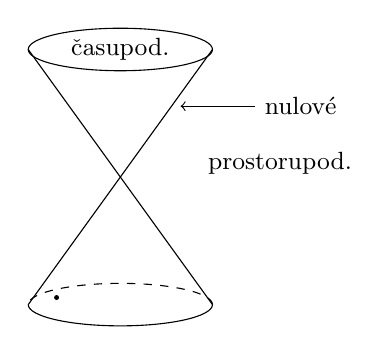
\begin{tikzpicture}[scale=0.9]
  % světelný kužel
  \draw (-1.3,1.8) -- (1.3,-1.8);
  \draw (1.3,1.8) -- (-1.3,-1.8);
  \draw (0,1.8) ellipse (1.3 and 0.3);
  \draw (-1.3,-1.8) arc (180:360:1.3 and 0.3);
  \draw[dashed] (1.3,-1.8) arc (0:180:1.3 and 0.3);
  \node at (0,1.8) {\small časupod.};
  \draw[->] (1.9,1.0) node[right] {\small nulové} -- (0.85,1.0);
  \node[right] at (1.1,0.2) {\small prostorupod.};
  \fill (-0.9,-1.7) circle (1pt);
\end{tikzpicture}
\end{minipage}

\kw{pseudoskal.\ součin}
\[ (a,b) = a^{\underline{n}}b^{\underline{m}}g_{\underline{nm}} \]
velikost
\begin{align*}
  a^2 &= (a,a) = a^{\underline{n}}a^{\underline{m}}g_{\underline{nm}} \in\mathbb{R} \quad\text{kv.\ velikosti} \\
  |a| &= |a^2|^{1/2} = |a^{\underline{n}}a^{\underline{m}}g_{\underline{nm}}|^{1/2}
\end{align*}

\begin{vysvetleni}[Lorentzovská metrika a kauzalita]
Lorentzovská metrika je modelem prostoročasu: v ortonormální bázi je $g=\operatorname{diag}(-1,1,\dots,1)$, tj.\ Minkowského metrika (s $c=1$). Nulové vektory tvoří \emph{světelný kužel}. Časupodobné vektory leží uvnitř kuželu a tvoří dvě konvexní složky (budoucí a minulá). Dva neprostorupodobné vektory jsou shodně orientované, právě když $(a,b)<0$.
Kauzální orientovatelnost znamená, že volbu \uv{budoucí} poloviny kužele lze provést spojitě po celé varietě.
Kvadrát velikosti $a^2$ může být záporný, proto se velikost definuje přes absolutní hodnotu. Pseudoskalární součin není pozitivně definitní a nulový vektor je kolmý sám na sebe.
Viz Krtouš, def.~D6.5--D6.7.
\end{vysvetleni}

\begin{minipage}{0.6\textwidth}
\kw{pseudosféry}
\begin{itemize}[nosep]
  \item[] časupodobné ps.-sf. \quad $a^2 = 1$
  \item[] prostorupodobné ps.-sf. \quad $n^2 = -1$
\end{itemize}
\pozn{přiřazení názvů odpovídá obrázkům: $a$ na jednodílném, $n$ na dvoudílném hyperboloidu}
\end{minipage}
\hfill
\begin{minipage}{0.38\textwidth}
\begin{tikzpicture}[scale=0.7,>=Stealth]
  % jednodílný hyperboloid
  \draw (0,1.5) ellipse (1.1 and 0.25);
  \draw (-1.1,1.5) .. controls (-0.45,0.5) and (-0.45,-0.5) .. (-1.1,-1.5);
  \draw (1.1,1.5) .. controls (0.45,0.5) and (0.45,-0.5) .. (1.1,-1.5);
  \draw (-1.1,-1.5) arc (180:360:1.1 and 0.25);
  \draw[dashed] (-0.55,0) arc (180:360:0.55 and 0.12);
  \fill (0,0) circle (1.5pt);
  \draw[->] (0,0) -- (0.62,0.45) node[right] {$a$};
  % dvoudílný hyperboloid
  \begin{scope}[xshift=3cm]
    \draw (-1.1,1.6) -- (1.1,-1.6); \draw (1.1,1.6) -- (-1.1,-1.6);
    \draw (0,1.6) ellipse (1.1 and 0.25);
    \draw (-1.1,1.6) .. controls (-0.5,0.7) and (0.5,0.7) .. (1.1,1.6);
    \draw (-1.1,-1.6) .. controls (-0.5,-0.7) and (0.5,-0.7) .. (1.1,-1.6);
    \draw (-1.1,-1.6) arc (180:360:1.1 and 0.25);
    \fill (0,0) circle (1.5pt);
    \draw[->] (0,0) -- (0,0.88) node[right] {$n$};
  \end{scope}
\end{tikzpicture}
\end{minipage}

lineární podprostory
\begin{itemize}[nosep]
  \item[] pouze prost.-pod.\ vekt.\ $\Rightarrow$ prostorupodobný
  \item[] právě jeden nulový vekt.\ $\Rightarrow$ nulový (světelný)
  \item[] alespoň jeden časupod.\ $\Rightarrow$ časupodobný
\end{itemize}

\begin{vysvetleni}[Pseudosféry a podprostory]
Pseudosféra $\{a: a^2=1\}$ je tvořena \emph{prostorupodobnými} jednotkovými vektory a je to jednodílný hyperboloid. Jako nadplocha má ale lorentzovskou indukovanou metriku (de Sitterův prostor), proto ji poznámky nazývají \uv{časupodobná}.
Pseudosféra $\{n: n^2=-1\}$ je tvořena časupodobnými jednotkovými vektory a je to dvoudílný hyperboloid (jedna slupka pro budoucí, druhá pro minulé vektory). Její indukovaná metrika je riemannovská (hyperbolický prostor), proto je \uv{prostorupodobná}.
Krtouš (odd.~6.2) pojmenovává pseudokružnice naopak podle charakteru vektorů, které je tvoří.
Klasifikace podprostorů (Krtouš, def.~D6.5): \uv{právě jeden nulový vektor} znamená jeden nulový \emph{směr}, ostatní vektory jsou prostorupodobné. Takový podprostor je tečný ke světelnému kuželu.
\end{vysvetleni}

%----------------------------------------------------------------------
\strana{GMI-08-6}
\pozn{Metr 5}

\begin{minipage}{0.6\textwidth}
\kw{pseudokružnice}
\begin{itemize}[nosep]
  \item[] rovina napnutá na ortonorm.\ bázi $t$, $q$ \\
          \quad $t^2 = -1 \qquad q^2 = 1 \qquad (t,q) = 0$
  \item[] pseudokruž.:
\end{itemize}
\[
  a^2 = 1 \qquad \vzorec{a = \pm(\operatorname{sh}\tau\ t + \operatorname{ch}\tau\ q)}
\]
\[
  n^2 = -1 \qquad \vzorec{n = \pm(\operatorname{ch}\beta\ t + \operatorname{sh}\beta\ q)}
\]
úkol: spočítejte délku pseudokružnice \\
\quad $\to$ přímo param.\ $\tau$ a $\beta$
\end{minipage}
\hfill
\begin{minipage}{0.37\textwidth}
\begin{tikzpicture}[scale=0.75,>=Stealth]
  % prostorupodobná pseudokružnice (pravá a levá větev)
  \draw[gray] (-2,-2) -- (2,2); \draw[gray] (-2,2) -- (2,-2);
  \draw[->] (-2.1,0) -- (2.2,0); \draw[->] (0,-2) -- (0,2.1);
  \draw[thick,domain=-1.3:1.3,samples=40] plot ({cosh(\x)},{sinh(\x)});
  \draw[thick,domain=-1.3:1.3,samples=40] plot ({-cosh(\x)},{sinh(\x)});
  \draw[->,very thick] (0,0) -- (0,1) node[left] {\small $t$};
  \draw[->,very thick] (0,0) -- (1,0) node[below] {\small $q$};
  \draw[->] (0,0) -- ({cosh(0.6)},{sinh(0.6)}) node[right] {\small $a$};
  \node at (1.38,0.3) {\small $\tau$};
  % časupodobná pseudokružnice
  \begin{scope}[yshift=-4.6cm]
    \draw[gray] (-2,-2) -- (2,2); \draw[gray] (-2,2) -- (2,-2);
    \draw[->] (-2.1,0) -- (2.2,0); \draw[->] (0,-2) -- (0,2.1);
    \draw[thick,domain=-1.3:1.3,samples=40] plot ({sinh(\x)},{cosh(\x)});
    \draw[thick,domain=-1.3:1.3,samples=40] plot ({sinh(\x)},{-cosh(\x)});
    \draw[->,very thick] (0,0) -- (0,1) node[left] {\small $t$};
    \draw[->,very thick] (0,0) -- (1,0) node[below] {\small $q$};
    \draw[->] (0,0) -- ({sinh(0.55)},{cosh(0.55)}) node[right] {\small $n$};
    \node at (0.3,1.35) {\small $\beta$};
  \end{scope}
\end{tikzpicture}
\end{minipage}

\subsubsection*{Pseudoúhly a úhly}
\begin{minipage}{0.55\textwidth}
obal $a,b$ prostorupodobný
\[
  \cos\underbrace{\sphericalangle a,b}_{\text{úhel }\gamma} = \frac{(a,b)}{|a|\,|b|}
\]
obal prostorupod.\ $a,b$ časupod.
\[
  \operatorname{ch}\underbrace{\sphericalangle a,b}_{\text{pseudoúhel }\tau} = \pm\frac{(a,b)}{|a|\,|b|}
\]
shodně orient.\ časupod.\ $a,b$
\[
  \operatorname{ch}\underbrace{\sphericalangle a,b}_{\text{rapidita }\beta} = -\frac{(a,b)}{|a|\,|b|}
\]
\end{minipage}
\hfill
\begin{minipage}{0.43\textwidth}
\begin{tikzpicture}[scale=0.6,>=Stealth]
  % kužel s prostorupodobnou rovinou
  \draw (-1.6,2) -- (1.6,-2); \draw (1.6,2) -- (-1.6,-2);
  \draw (0,2) ellipse (1.6 and 0.35);
  \draw (-1.6,-2) arc (180:360:1.6 and 0.35);
  \draw[fill=gray!10,opacity=0.8] (-2.6,-0.6) -- (1.4,-1.2) -- (2.8,0.6) -- (-1.2,1.2) -- cycle;
  \draw[->] (0.2,0) -- (1.3,0.5) node[right] {\small $a$};
  \draw[->] (0.2,0) -- (1.4,0.05) node[right] {\small $b$};
  \node at (1.0,0.18) {\scriptsize $\gamma$};
  % časupodobné roviny: pseudoúhel tau (+ a -)
  \begin{scope}[yshift=-4.2cm,xshift=-1.6cm]
    \draw (-1.3,-1.6) -- (1.1,-1.3) -- (1.3,1.6) -- (-1.1,1.3) -- cycle;
    \draw[gray,dashed] (-1,-1) -- (1,1); \draw[gray,dashed] (-1,1) -- (1,-1);
    \draw[->] (0,0) -- (0.8,1.0) node[right] {\small $a$};
    \draw[->] (0,0) -- (0.9,-0.1) node[right] {\small $b$};
    \node at (0.62,0.35) {\scriptsize $\tau$};
    \node at (0,-2) {$+$};
  \end{scope}
  \begin{scope}[yshift=-4.2cm,xshift=1.6cm]
    \draw (-1.3,-1.6) -- (1.1,-1.3) -- (1.3,1.6) -- (-1.1,1.3) -- cycle;
    \draw[gray,dashed] (-1,-1) -- (1,1); \draw[gray,dashed] (-1,1) -- (1,-1);
    \draw[->] (0,0) -- (0.8,1.0) node[right] {\small $a$};
    \draw[->] (0,0) -- (-0.95,0) node[left] {\small $b$};
    \node at (0.62,0.35) {\scriptsize $\tau$};
    \node at (0,-2) {$-$};
  \end{scope}
  % rapidita beta
  \begin{scope}[yshift=-8.6cm,xshift=-1.6cm]
    \draw (-1.3,-1.6) -- (1.1,-1.3) -- (1.3,1.6) -- (-1.1,1.3) -- cycle;
    \draw[gray,dashed] (-1,-1) -- (1,1); \draw[gray,dashed] (-1,1) -- (1,-1);
    \draw[->] (0,-0.6) -- (-0.35,0.8) node[left] {\small $a$};
    \draw[->] (0,-0.6) -- (0.45,0.95) node[right] {\small $b$};
    \node at (0.02,0.35) {\scriptsize $\beta$};
  \end{scope}
\end{tikzpicture}
\end{minipage}

\begin{vysvetleni}[Pseudokružnice, pseudoúhly a rapidita]
V rovině s lorentzovskou metrikou a ortonormální bází $t,q$ hrají roli kružnice hyperboly. Parametry $\tau$, $\beta$ v $a=\pm(\operatorname{sh}\tau\,t+\operatorname{ch}\tau\,q)$, $n=\pm(\operatorname{ch}\beta\,t+\operatorname{sh}\beta\,q)$ jsou přímo lorentzovské délky oblouku pseudokružnice měřené od $q$, resp.\ od $t$. To je řešení úkolu: $\big|\frac{\mathrm{d}a}{\mathrm{d}\tau}\big|=1$, takže délka oblouku je $\Delta\tau$ (celá větev má nekonečnou délku). Proto jsou $\tau$, $\beta$ vhodnou analogií úhlu.
Pro shodně orientované časupodobné $a,b$ je $(a,b)<0$, odtud znaménko $-$ u rapidity. Ve speciální relativitě je $\beta$ rapidita vzájemného pohybu dvou pozorovatelů se čtyřrychlostmi $a,b$: $v=\operatorname{th}\beta$ a $\operatorname{ch}\beta=\gamma_{\text{Lor}}=(1-v^2)^{-1/2}$. Rapidity se při skládání pohybů v jednom směru sčítají.
Znaménko $\pm$ u pseudoúhlu se volí tak, aby pravá strana byla $\geq1$. Znaménko $-$ nastává, když $a$ a $b$ leží v protilehlých oblastech vně světelného kuželu (obrázek).
Viz Krtouš, vztahy (6.2)--(6.4), def.~D6.8.
\end{vysvetleni}

%----------------------------------------------------------------------
\strana{GMI-08-7}
\subsection{Délka křivky} \pozn{Met-6}

\kw{kauzální charakter křivky} $z(\tau)$
\begin{itemize}[nosep]
  \item[--] dán znaménkem kv.\ velikosti tečného vektoru
\end{itemize}
\[
  \frac{\mathrm{D}z^{\underline{a}}}{\mathrm{d}\tau}\frac{\mathrm{D}z^{\underline{b}}}{\mathrm{d}\tau}\,g_{\underline{ab}} \lesseqgtr 0
  \qquad
  \begin{array}{cl}
    < & \text{časupod.\ kř.} \\
    = & \text{nulová/světelná kř.} \\
    > & \text{prostorupod.\ kř.}
  \end{array}
\]
budeme uvažovat pouze kř., jejichž kauzální char.\ se nemění

\begin{definice}[Délka křivky]
\[
  \vzorec{\Delta s = \int_{(\tau_z,\tau_k)}\Big|\frac{\mathrm{D}z^{\underline{a}}}{\mathrm{d}\tau}\frac{\mathrm{D}z^{\underline{b}}}{\mathrm{d}\tau}g_{\underline{ab}}\Big|^{1/2}\mathrm{d}\tau
  = \int_{(\tau_z,\tau_k)}\Big|\frac{\mathrm{D}z}{\mathrm{d}\tau}\Big|\,\mathrm{d}\tau = \int_{(\tau_z,\tau_k)}\mathrm{d}s}
\]
\end{definice}
\begin{itemize}[nosep]
  \item[] nezávisí na parametrizaci křivky
  \item[] abs.\ hodn.\ se uplatňuje pro časupod.\ kř.
  \item[] svět.\ kř.\ mají nulovou délku
\end{itemize}

\begin{vysvetleni}[Délka křivky]
$\frac{\mathrm{D}z}{\mathrm{d}\tau}$ je tečný vektor ke křivce $z(\tau)$. Integrál je invariantní vůči reparametrizaci, protože při $\tau\to\tau'(\tau)$ se tečný vektor násobí $\frac{\mathrm{d}\tau}{\mathrm{d}\tau'}$ a $\mathrm{d}\tau'=\frac{\mathrm{d}\tau'}{\mathrm{d}\tau}\mathrm{d}\tau$.
Pro riemannovskou metriku dostaneme obyčejnou délku. Pro lorentzovskou metriku dostaneme u prostorupodobných křivek vlastní délku a u časupodobných \emph{vlastní čas} pozorovatele $\Delta s=\int\sqrt{-g_{ab}\dot z^a\dot z^b}\,\mathrm{d}\tau$, což je čas naměřený hodinami nesenými podél křivky.
Viz Krtouš, def.~D6.12.
\end{vysvetleni}

\kw{kauzální vztah bodů} \quad (kauzálně orient.\ variety!)

\begin{minipage}{0.68\textwidth}
\begin{itemize}[nosep]
  \item[] $x$ je v budoucnu $y$ \quad $(x > y)$ \\
          \quad $\Leftrightarrow$ existuje časupod.\ kř.\ z $y$ do $x$
  \item[] $x,y$ časupodobně polož.\ \quad $(x\not\sim y)$ \\
          \quad $\Leftrightarrow$ $x > y$ nebo $y > x$
  \item[] $x,y$ prostorupodobně polož.\ \quad $(x\sim y)$ \\
          \quad $\Leftrightarrow$ neexistuje časupod.\ kř.\ spojující $x$ -- $y$
\end{itemize}
\end{minipage}
\hfill
\begin{minipage}{0.3\textwidth}
\pozor{pozor:} pro časupod.\ polož.\ body existuje prostorup.\ kř.

\centering
\begin{tikzpicture}[scale=0.7,>=Stealth]
  \node[below] at (0,0) {\small $x$};
  \node[above] at (0,2.2) {\small $y$};
  \draw[->] (0,0) .. controls (0.6,0.2) and (0.6,0.4) .. (0,0.5)
             .. controls (-0.4,0.6) and (0.6,0.8) .. (0.5,1.0)
             .. controls (0.4,1.2) and (-0.4,1.2) .. (0.3,1.5)
             .. controls (0.8,1.7) and (0.5,2.0) .. (0,2.2);
\end{tikzpicture}
\end{minipage}

\kw{vzdálenost bodů}
\begin{itemize}[nosep]
  \item[] kauzálně orient.\ var.\ bez uzavř.\ čas.\ smyček
  \item[] vzdálenost je extremální délka křivky daného kauz.\ typu
\end{itemize}
\begin{align*}
  x\sim y &\qquad \text{vzdálenost} = \text{\sout{minimální délka}}\ \text{délka extremální prostorupod.\ kř.} \\
  x\not\sim y &\qquad \text{časový separ.} = \text{maximální délka časupod.\ kř.}
\end{align*}

\begin{minipage}{0.66\textwidth}
je potřeba uvažovat lokální extrém
\begin{itemize}[nosep]
  \item[--] může vést na víceznačnou vzdálenost
  \item[--] pro prostorupod.\ kř.\ je prostorupod.\ geodetika nestabilní extrém (sedlový bod) $\to$ \sout{délka} není minimální
\end{itemize}
\end{minipage}
\hfill
\begin{minipage}{0.32\textwidth}
\begin{tikzpicture}[scale=0.8,>=Stealth]
  \foreach \x in {-0.5,0.5,1.5} { \draw[gray!60] (\x,-0.9) -- (\x,0.9); }
  \draw[gray!60] (-1,0) -- (2.4,0);
  \draw[gray!60] (-0.6,-0.6) -- (0.6,0.6); \draw[gray!60] (-0.6,0.6) -- (0.6,-0.6);
  \fill (-0.5,0) circle (1.5pt); \fill (1.5,0) circle (1.5pt);
  \draw[thick] (-0.5,0) -- (1.5,0);
  \draw[thick] (-0.5,0) -- (0.5,0.5) -- (1.5,0);
  \draw[thick] (-0.5,0) -- (0.2,-0.3) -- (1.5,0);
  \draw[<-] (0.6,0.47) -- (1.6,0.95) node[right] {\scriptsize kratší};
  \draw[<-] (0.9,0.02) -- (1.9,0.55) node[right] {\scriptsize geod.};
  \draw[<-] (0.8,-0.18) -- (1.4,-0.7) node[right] {\scriptsize delší};
\end{tikzpicture}
\end{minipage}

\begin{vysvetleni}[Kauzalita a vzdálenost v lorentzovské geometrii]
Časupodobnou křivku lze libovolně \uv{zkrátit} tím, že ji nahradíme blízkou křivkou zubatou, skoro světelnou. Infimum délek časupodobných křivek je proto $0$ a smysl má jen \emph{maximum}: časupodobná geodetika maximalizuje (lokálně) vlastní čas. To je podstata paradoxu dvojčat, kde je déle žijící dvojče to inerciální.
Naopak mezi prostorupodobně položenými body lze délku prostorupodobné křivky změnit oběma směry (obrázek: výchylka v časovém směru zkracuje, v prostorovém prodlužuje). Prostorupodobná geodetika je tedy sedlový bod, ne minimum. Proto se vzdálenost definuje jako délka \emph{extremální} křivky a může být víceznačná.
Podmínka \uv{bez uzavřených časupodobných smyček} zajišťuje, že vztah \uv{$x$ je v budoucnosti $y$} je rozumné uspořádání.
\end{vysvetleni}

%----------------------------------------------------------------------
\strana{GMI-08-8}
\subsection{Levi-Civitův tenzor a Hodgeův duál} \pozn{Met-7}

totálně a-sym.\ formy \quad $\Lambda^dM$
\begin{itemize}[nosep]
  \item[--] jednodim.\ prostor
  \item[--] metrika umožňuje vybrat \uv{jednotku}
\end{itemize}

\begin{definice}[Levi-Civitův tenzor]
\begin{align*}
  &\varepsilon_{\underline{a}_1\dots\underline{a}_d}\in\Lambda^dM \\
  &\varepsilon_{\underline{a}_1\dots\underline{a}_d}\,{}^\sharp\varepsilon^{\underline{a}_1\dots\underline{a}_d} = (\operatorname{sign}g)\,d!
    \qquad\text{tj.}\qquad \vzorec{\varepsilon\bullet{}^\sharp\varepsilon = \operatorname{sign}g} \\
  &\varepsilon_{1\dots d} > 0 \quad \text{vzhledem k pos.\ orient.\ bázi}
\end{align*}
\end{definice}

\kw{orientace bází}
\begin{itemize}[nosep]
  \item[] $e_k$, $e'_k$ shodně orient., pokud přech.\ matice $M^k{}_l$ má kladný determinant \quad $\det M > 0$
  \item[$\Downarrow$] dvě třídy bází (v každém bodě) \\
          \quad jednu nazveme pos.\ orient., druhou neg.\ orient.
  \item[] varieta je \kw{orientovatelná}, pokud lze zvolit pos.\ orient.\ báze globálně spojitě
\end{itemize}

ortonormální báze
\begin{align*}
  {}^\sharp\varepsilon^{1\dots d} &= g^{1a_1}\cdots g^{da_d}\varepsilon_{a_1\dots a_d} = g^{11}\cdots g^{dd}\varepsilon_{1\dots d} = (\operatorname{sign}g)\,\varepsilon_{1\dots d} \\
  \varepsilon_{1\dots d}\,{}^\sharp\varepsilon^{1\dots d} &= \operatorname{sign}g\,(\varepsilon_{1\dots d})^2 = \operatorname{sign}g \ \Rightarrow\ \varepsilon_{1\dots d} = \pm1 \\
  \Rightarrow\ &\vzorec{\varepsilon = e^1\wedge\dots\wedge e^d} \qquad \text{pro pos.\ orient.\ ortonorm.\ bázi}
\end{align*}

obecná báze
\begin{align*}
  {}^\sharp\varepsilon^{1\dots d} &= g^{1a_1}\cdots g^{da_d}\varepsilon_{a_1\dots a_d} = (\det g^{ab})\,\varepsilon_{1\dots d} \\
  \varepsilon_{1\dots d}\,{}^\sharp\varepsilon^{1\dots d} &= (\det g^{ab})(\varepsilon_{1\dots d})^2 = (\det g_{ab})^{-1}(\varepsilon_{1\dots d})^2 = \operatorname{sign}g \\
  \Rightarrow\ \vzorec{\varepsilon_{1\dots d} = \pm|\det g_{ab}|^{1/2}} &\qquad \text{díky } \operatorname{sign}\det g_{ab} = \operatorname{sign}g
\end{align*}

inverze Levi-Civit.\ tenz.
\[
  \varepsilon^{-1} = \operatorname{sign}g\ {}^\sharp\varepsilon
  \qquad\Leftarrow\qquad \varepsilon^{-1\,1\dots d} = (\varepsilon_{1\dots d})^{-1} \qquad {}^\sharp\varepsilon^{1\dots d} = \oprava{\operatorname{sign}g\,|\varepsilon_{1\dots d}|^{-1}}{|\varepsilon_{1\dots d}|^{-1}}
\]
vztah k AS jednotce
\[
  {}^\sharp\varepsilon^{\underline{a}_1\dots\underline{a}_d}\,\varepsilon_{\underline{b}_1\dots\underline{b}_d} = d!\,\operatorname{sign}g\ {}^{[d]}\delta^{\underline{a}_1\dots\underline{a}_d}_{\underline{b}_1\dots\underline{b}_d}
  \qquad
  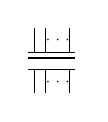
\begin{tikzpicture}[baseline=-2pt,scale=0.5]
    \draw (-0.6,0.15) -- (0.6,0.15); \draw (-0.6,0.3) -- (0.6,0.3);
    \foreach \x in {-0.45,-0.15,0.45} \draw (\x,0.3) -- (\x,0.9);
    \node at (0.15,0.6) {\tiny$\cdots$};
    \draw (-0.6,-0.15) -- (0.6,-0.15);
    \foreach \x in {-0.45,-0.15,0.45} \draw (\x,-0.15) -- (\x,-0.75);
    \node at (0.15,-0.45) {\tiny$\cdots$};
  \end{tikzpicture}
  = (\operatorname{sign}g)\,d!\
  \begin{tikzpicture}[baseline=-2pt,scale=0.5]
    \foreach \x in {-0.3,0,0.3} \draw (\x,-0.7) -- (\x,0.7);
    \draw (-0.5,0) -- (0.5,0);
  \end{tikzpicture}
\]

\begin{vysvetleni}[Levi-Civitův tenzor]
Prostor $d$-forem je jednorozměrný, takže $d$-forma je určena jedním číslem $\varepsilon_{1\dots d}$. Metrika (normalizace) a orientace (znaménko) z něj vyberou jednu význačnou, \emph{objemovou formu} $\varepsilon$. Hodnota $\varepsilon(e_1,\dots,e_d)$ je orientovaný objem rovnoběžnostěnu napnutého na vektory, v kladně orientovaných souřadnicích $\varepsilon=|\det g_{ab}|^{1/2}\,\mathrm{d}x^1\wedge\dots\wedge\mathrm{d}x^d$ (v $\mathbb{R}^3$ ve sférických souřadnicích $r^2\sin\theta\,\mathrm{d}r\wedge\mathrm{d}\theta\wedge\mathrm{d}\varphi$).
Tečka $\bullet$ značí úplné zúžení antisymetrických tenzorů s faktorem $\frac1{p!}$, tj.\ $\omega\bullet\sigma=\frac1{p!}\omega_{a_1\dots a_p}\sigma^{a_1\dots a_p}$.
Tenzor se zvednutými indexy ${}^\sharp\varepsilon$ a inverze $\varepsilon^{-1}$ (definovaná $\varepsilon^{-1}\bullet\varepsilon=1$) se liší o $\operatorname{sign}g$, v lorentzovském případě tedy o znaménko. V ortonormální bázi je $\varepsilon_{1\dots d}=1$, ale ${}^\sharp\varepsilon^{1\dots d}=\operatorname{sign}g$; odtud i opravené znaménko výše (viz řádek \uv{obecná báze}: ${}^\sharp\varepsilon^{1\dots d}=\det(g^{ab})\,\varepsilon_{1\dots d}$).
Diagram: dva vodorovné pruhy s nožičkami nahoru a dolů jsou ${}^\sharp\varepsilon$ a $\varepsilon$ s volnými indexy. Svislé čáry přeškrtnuté vodorovnou čarou značí antisymetrizovaný součin delt ${}^{[d]}\delta=\delta^{[a_1}_{b_1}\cdots\delta^{a_d]}_{b_d}$ (\uv{AS jednotka}).
Viz Krtouš, def.~D6.13, vztahy (6.13)--(6.16), lemma V6.3.
\end{vysvetleni}

%----------------------------------------------------------------------
\strana{GMI-08-9}
\subsubsection*{Hodgeův duál} \pozn{Met-8}
\begin{definice}[Hodgeův duál]
\begin{align*}
  &*:\ \Lambda^pM \to \Lambda^{d-p}M \\
  &(*\omega)_{\underline{a}_{p+1}\dots\underline{a}_d} = \frac{1}{p!}\,{}^\sharp\omega^{\underline{b}_1\dots\underline{b}_p}\,\varepsilon_{\underline{b}_1\dots\underline{b}_p\underline{a}_{p+1}\dots\underline{a}_d}
   = \vzorec{{}^\sharp\omega\bullet\varepsilon}
\end{align*}
\end{definice}

platí
\[
  \vzorec{**\omega = \operatorname{sign}g\,(-1)^{p(d-p)}\,\omega}
\]
\begin{align*}
  (**\omega)_{\underline{a}_1\dots\underline{a}_p}
  &= \frac{1}{(d-p)!}(*\omega)^{\underline{n}_1\dots\underline{n}_{d-p}}\,\varepsilon_{\underline{n}_1\dots\underline{n}_{d-p}\underline{a}_1\dots\underline{a}_p} = \\
  &= \frac{1}{p!\,(d-p)!}\,\omega_{\underline{b}_1\dots\underline{b}_p}\,\varepsilon^{\underline{b}_1\dots\underline{b}_p\underline{n}_1\dots\underline{n}_{d-p}}\,\varepsilon_{\underline{a}_1\dots\underline{a}_p\underline{n}_1\dots\underline{n}_{d-p}}\,(-1)^{p(d-p)} \\
  &= \operatorname{sign}g\,(-1)^{p(d-p)}\,\frac{d!}{p!\,(d-p)!}\,\omega_{\underline{b}_1\dots\underline{b}_p}\,{}^{[d]}\delta^{\underline{b}_1\dots\underline{b}_p\underline{n}_1\dots\underline{n}_{d-p}}_{\underline{a}_1\dots\underline{a}_p\underline{n}_1\dots\underline{n}_{d-p}} \\
  &= \operatorname{sign}g\,(-1)^{p(d-p)}\,{}^{[p]}\delta^{\underline{b}_1\dots\underline{b}_p}_{\underline{a}_1\dots\underline{a}_p}\,\omega_{\underline{b}_1\dots\underline{b}_p} \\
  &= \operatorname{sign}g\,(-1)^{p(d-p)}\,\omega_{\underline{a}_1\dots\underline{a}_p}
\end{align*}

\begin{vysvetleni}[Hodgeův duál]
$*$ přiřadí $p$-formě \uv{doplňkovou} $(d-p)$-formu. Rovinný element $p$-formy se zobrazí na kolmý doplněk, např.\ ve $\mathbb{R}^3$: $*1=\varepsilon$, $*\mathrm{d}x=\mathrm{d}y\wedge\mathrm{d}z$, $*(\mathrm{d}x\wedge\mathrm{d}y)=\mathrm{d}z$. Obecně v ortonormální bázi $*(e^1\wedge\dots\wedge e^p)=\pm e^{p+1}\wedge\dots\wedge e^d$, kde znaménko je součin kvadrátů velikostí $e^1,\dots,e^p$.
V důkazu $**$ se nejdřív přesunou indexy $\underline{a}$ v $\varepsilon$ dopředu, což dá $(-1)^{p(d-p)}$. Pak se použije zúžení dvou Levi-Civitových tenzorů přes $d-p$ indexů, ${}^\sharp\varepsilon^{b_1\dots b_p n\dots}\varepsilon_{a_1\dots a_p n\dots}=\operatorname{sign}g\,p!\,(d-p)!\,{}^{[p]}\delta^{b_1\dots b_p}_{a_1\dots a_p}$ (Krtouš, (6.16)).
Viz Krtouš, def.~D6.14, lemma V6.5.
\end{vysvetleni}

%----------------------------------------------------------------------
\strana{GMI-08-10}
\subsubsection*{(Pseudo)skal.\ součin na formách} \pozn{Met-9}
$\omega,\sigma\in\Lambda^pM$
\begin{align*}
  \omega\bullet\sigma &= \omega\bullet{}^\sharp\sigma = \frac{1}{p!}\,\omega_{\underline{a}_1\dots\underline{a}_p}\sigma^{\underline{a}_1\dots\underline{a}_p} = \sum_{a_1<\dots<a_p}\omega_{a_1\dots a_p}\sigma^{a_1\dots a_p} \\
  \omega^2 &= \omega\bullet\omega
\end{align*}
\quad signatura závisí na signatuře $g$ a stupni $p$

vlastnosti Hodgeho duálu
\[
  \vzorec{(*\omega)\bullet(*\sigma) = (\operatorname{sign}g)\,\omega\bullet\sigma}
\]
\begin{align*}
  \text{Důk.}\quad (*\omega)\bullet(*\sigma) &= \frac{1}{(d-p)!}\frac{1}{p!}\frac{1}{p!}\,\omega_{\underline{a}_1\dots\underline{a}_p}\varepsilon^{\underline{a}_1\dots\underline{a}_p\underline{n}_{p+1}\dots\underline{n}_d}\,\sigma^{\underline{b}_1\dots\underline{b}_p}\varepsilon_{\underline{b}_1\dots\underline{b}_p\underline{n}_{p+1}\dots\underline{n}_d} \\
  &= \operatorname{sign}g\,\frac{p!}{p!\,p!}\,\omega_{\underline{a}_1\dots\underline{a}_p}\sigma^{\underline{b}_1\dots\underline{b}_p}\,{}^{[p]}\delta^{\underline{a}_1\dots\underline{a}_p}_{\underline{b}_1\dots\underline{b}_p}
   = \operatorname{sign}g\,\frac{1}{p!}\,\omega_{\underline{a}_1\dots\underline{a}_p}\sigma^{\underline{a}_1\dots\underline{a}_p} \\
  &= \operatorname{sign}g\ \omega\bullet\sigma
\end{align*}
\[
  \vzorec{\omega\wedge*\sigma = \sigma\wedge*\omega = \omega\bullet\sigma\ \varepsilon = *(\omega\bullet\sigma)}
\]
\begin{align*}
  \text{Důk.}\quad *(\omega\wedge*\sigma) &= \frac{1}{d!}\frac{d!}{p!\,(d-p)!}\frac{1}{p!}\,\omega_{\underline{a}_1\dots\underline{a}_p}\sigma^{\underline{b}_1\dots\underline{b}_p}\varepsilon_{[\underline{b}_1\dots\underline{b}_p|\underline{a}_{p+1}\dots\underline{a}_d]}\varepsilon^{\underline{a}_1\dots\underline{a}_d} \\
  &= \frac{\operatorname{sign}g}{p!}\,\omega_{\underline{a}_1\dots\underline{a}_p}\sigma^{\underline{a}_1\dots\underline{a}_p} = \operatorname{sign}g\ \omega\bullet\sigma \\
  *(\omega\bullet\sigma) &= \operatorname{sign}g\,**(\omega\wedge*\sigma) = (\operatorname{sign}g)^2(-1)^{0d}\,\omega\wedge*\sigma = \omega\wedge*\sigma = \omega\bullet\sigma\ \varepsilon
\end{align*}
\[
  \omega\wedge*\omega = \omega^2\,\varepsilon = *\omega^2
\]

\begin{vysvetleni}[Skalární součin forem a $\omega\wedge*\sigma$]
$\omega\bullet\sigma$ je součin indukovaný metrikou na $\Lambda^pM$. Faktor $\frac1{p!}$ zajistí, že se každá nezávislá složka započte jednou, takže v ortonormální bázi riemannovské metriky je $\{e^{a_1}\wedge\dots\wedge e^{a_p}\}_{a_1<\dots<a_p}$ ortonormální báze $\Lambda^pM$. Pro smíšenou signaturu tento součin není definitní.
Vztah $\omega\wedge*\sigma=(\omega\bullet\sigma)\,\varepsilon$ dovoluje zapsat \uv{kvadratické} výrazy jako $d$-formy, které lze integrovat. Například lagrangián elektromagnetického pole je úměrný $F\wedge*F=F^2\varepsilon$, kde $F^2=\frac12F_{ab}F^{ab}$.
V dokazovaných krocích se opět používá zúžení ${}^\sharp\varepsilon\,\varepsilon$ přes $d-p$ indexů. Nula v exponentu $(-1)^{0d}$ připomíná, že $\omega\bullet\sigma$ je 0-forma.
Viz Krtouš, def.~D6.15, lemma V6.6.
\end{vysvetleni}

\begin{priklad}[příklady]
$d = 2$ \quad $(+\,+)$
\begin{align*}
  **\omega &= \omega & \omega&\in\Lambda^pM \quad p = 0,2 \\
  **\alpha &= -\alpha & \alpha&\in\Lambda^1M \\
  |*\alpha| &= |\alpha| && \Leftarrow\ \varepsilon^a{}_n\varepsilon^b{}_m g_{ab} = g_{nm} \\
  (*\alpha)\cdot g\cdot\alpha &= 0 && \Leftarrow\ \alpha^m\alpha^n\varepsilon^k{}_m g_{kn} = 0
\end{align*}
$d = 3$ \quad $(+\,+\,+)$
\[
  **\omega = \omega \qquad \omega\in\Lambda^pM \quad p = 0,1,2,3
\]
$d = 4$ \quad $(-\,+\,+\,+)$
\begin{align*}
  **\omega &= \omega & \omega&\in\Lambda^pM \quad p = 1,3 \\
  **\omega &= -\omega & & p = 0,2,4
\end{align*}
\quad $*$ definuje na $\Lambda^2M$ komplexní strukturu, tj.\ $*:\Lambda^2M\to\Lambda^2M$, \ $*^2 = -\mathrm{id}$
\end{priklad}

\kw{vektorové násobení} \quad $d = 3$
\begin{align*}
  a\times b &= *(a\wedge b) && \text{(automat.\ sníž.\ indexů)} \\
  (a\times b)^n &= \tfrac12(a\wedge b)_{kl}\varepsilon^{kln} = a^kb^l\varepsilon^{kln} && \checkmark
\end{align*}

\begin{vysvetleni}[K příkladům]
Všechny případy plynou z $**=\operatorname{sign}g\,(-1)^{p(d-p)}$. V lichých dimenzích je $p(d-p)$ vždy sudé. V $d=2$ (riemannovsky) je $*$ na 1-formách otočení o pravý úhel: zachovává velikost a dává kolmý vektor, a $**=-1$ odpovídá otočení o $\pi$.
V $d=4$ s lorentzovskou signaturou je na 2-formách $*^2=-1$, takže $*$ se chová jako imaginární jednotka. Vlastní hodnoty jsou $\pm\mathrm{i}$ a 2-formy (např.\ tenzor elektromagnetického pole $F$) se dají rozložit na komplexní \emph{samoduální} a \emph{antisamoduální} části, $F\mp\mathrm{i}*F$. Dualita $F\mapsto*F$ zaměňuje $\vec E$ a $\vec B$ (až na znaménko).
Vektorový součin: v $\mathbb{R}^3$ je $a\wedge b$ \uv{orientovaná ploška} a její duál je normálový vektor $a\times b$. Krtouš, příklady P6.1, P6.2.
\end{vysvetleni}

%----------------------------------------------------------------------
\strana{GMI-08-11}
\subsection{Killingovy vektory} \pozn{Met-10}

\kw{symetrie metriky} \\
\quad $=$ diffeomorfismus zachovávající metriku \quad $\phi_*g = g$

spojitá symetrie metriky \quad $\phi_{\tau*}g = g$ \qquad $\phi_\tau$ tok

\begin{definice}[Killingův vektor]
diferenciální vyjádření
\[
  \vzorec{\mathcal{L}_\xi g = 0} \qquad \xi \text{ generátor toku } \phi_\tau
\]
$\xi$ \ \kw{Killingův vektor}
\end{definice}

\begin{vysvetleni}[Killingovy vektory]
Killingův vektor je infinitezimální izometrie: posunutí bodů podél jeho toku nemění vzdálenosti. Podmínka $\mathcal{L}_\xi g=0$ je ve složkách $\xi^ng_{ab,n}+\xi^n{}_{,a}g_{nb}+\xi^n{}_{,b}g_{an}=0$. Pomocí Levi-Civitovy derivace (kap.\ Metrické derivace) ji lze zapsat jako \emph{Killingovu rovnici} $\nabla_a\xi_b+\nabla_b\xi_a=0$.
Příklad: rovina $\mathbb{R}^2$ s eukleidovskou metrikou má 3 nezávislé Killingovy vektory, $\partial_x$, $\partial_y$ (posunutí) a $x\partial_y-y\partial_x=\partial_\varphi$ (rotace). Pokud metrika nezávisí na souřadnici $x^1$, je $\partial_1$ Killingův vektor. Každý Killingův vektor dává zachovávající se veličinu podél geodetik, $u^a\xi_a=\text{konst}$.
Konformní Killingův vektor zachovává metriku jen až na násobek, tedy zachovává úhly a světelné kužele, ale ne délky.
Viz Krtouš, odd.~6.5, def.~D6.16, D6.17.
\end{vysvetleni}

\kw{konformní symetrie}
\[
  \phi_{\tau*}g = \Omega^2_\tau\,g \qquad\text{diferenciálně:}\qquad \mathcal{L}_\xi g = \lambda g
\]

\begin{veta}[algebra Killing.\ vektorů]
$\xi,\eta$ Kill.\ vekt.\ $\Rightarrow$ $[\xi,\eta]$ Kill.\ vekt. \\
$\xi,\eta$ konf.\ Kill.\ vekt.\ $\Rightarrow$ $[\xi,\eta]$ konf.\ Kill.\ vekt.
\end{veta}
Důk.\ \quad $\mathcal{L}_{[\xi,\eta]} = \mathcal{L}_\xi\mathcal{L}_\eta - \mathcal{L}_\eta\mathcal{L}_\xi$ \qquad
$\mathcal{L}_\eta g = 0,\ \mathcal{L}_\xi g = 0 \ \Rightarrow\ \mathcal{L}_{[\xi,\eta]}g = 0$

Důk.\ \quad $\mathcal{L}_\xi g = \kappa g$, \ $\mathcal{L}_\eta g = \lambda g$
\begin{align*}
  \mathcal{L}_{[\xi,\eta]}g &= \mathcal{L}_\xi\mathcal{L}_\eta g - \mathcal{L}_\eta\mathcal{L}_\xi g = \mathcal{L}_\xi(\lambda g) - \mathcal{L}_\eta(\kappa g) \\
  &= \kappa\lambda g + (\xi\cdot\mathrm{d}\lambda)g - \kappa\lambda g - (\eta\cdot\mathrm{d}\kappa)g = (\xi\cdot\mathrm{d}\lambda - \eta\cdot\mathrm{d}\kappa)\,g \qquad \checkmark
\end{align*}

\begin{vysvetleni}[Lieova algebra Killingových vektorů]
Díky identitě $\mathcal{L}_{[\xi,\eta]}=[\mathcal{L}_\xi,\mathcal{L}_\eta]$ a linearitě $\mathcal{L}_\xi$ v $\xi$ (pro konstantní koeficienty) tvoří Killingovy vektory \emph{Lieovu algebru}. Je to algebra grupy izometrií. Její dimenze je nejvýše $\frac{d(d+1)}{2}$ a maxima dosahují maximálně symetrické prostory: eukleidovský prostor, sféra, Minkowského prostor (Poincarého algebra, v $d=4$ dimenze 10).
V konformním případě se při výpočtu použil Leibniz $\mathcal{L}_\xi(\lambda g)=(\xi\cdot\mathrm{d}\lambda)g+\lambda\,\mathcal{L}_\xi g$. Krtouš, věta V6.7.
\end{vysvetleni}

